
\chapter{LED indicators}

\newcommand{\LEDX}{{\rule{0.4em}{1.0em}}}
\newcommand{\LEDO}{{\rule{0.4em}{0.1em}}}

\newcommand{\ShowColor}[1]{{\color{#1}\rule{2em}{0.8em}}}

Komar is equipped with five LEDs that indicate the status of the hardware and software.
Their positions are shown in the figure \ref{fig:characteristics_leds_placement} below.

\begin{figure}[!hbt]
    \centering
    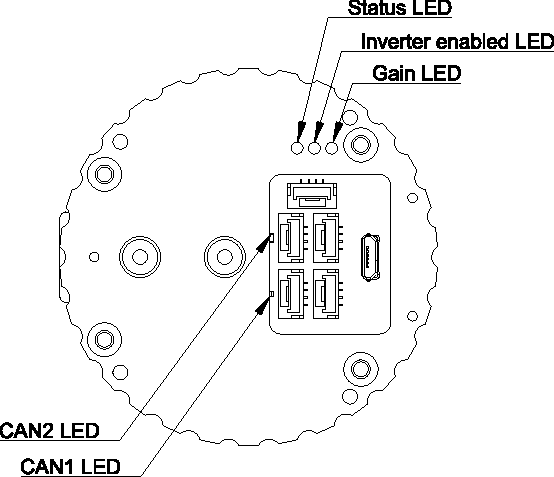
\includegraphics[width=0.7\textwidth]{figures/leds_placement}
    \caption{LEDs placement drawing\label{fig:characteristics_leds_placement}}
\end{figure}

\section{CAN LEDs}
The CAN1 and CAN2 LEDs indicate the flow of data through the CAN buses. It blinks in \textbf{green} once if
at least one CAN frame was successfully transmitted or received within the last 25 milliseconds. It
remains constantly \textbf{green} when the CAN traffic on the bus rises about 40 frames per second.

\section{Inverter enabled LED}
The Inverter enabled LED indicates that the power transistor driver scheme is enabled. When enabled, the LED
will illuminate in \textbf{orange}.

\section{Gain LED}
The Gain LED reflects the status of the automatic gain control (AGC) of the phase current measurement analog
front-end. When the LED is on, the gain is low; when off, it is high. The LED illuminates in \textbf{orange}.
\newpage
\section{Status LED}
The Status LED indicates the current state of the firmware. During boot-up, the LED will report
the firmware status as shown in table \ref{table:characteristics_status_led} below:

\begin{ZubaxSimpleTable}{Status LED during boot\label{table:characteristics_status_led}}{|l l X|}
    Color                     & Status                  & Description \\
    \ShowColor{yellow} Yellow & No application to boot  & The firmware has not been
    flashed to the ESC or the firmware has been damaged. \\
    \ShowColor{blue} Blue & Application being upgraded &  The application is in the process of being upgraded. \\
    \ShowColor{green} Green & Boot canceled & The device firmware has not been properly signed. \\
    \ShowColor{magenta} Magenta   & Ready to boot & The device has power but has yet to load the application. \\
\end{ZubaxSimpleTable}

During operation, the LED will report the status as shown in table \ref{table:characteristics_status_led_behavior}
below:

\begin{ZubaxSimpleTable}{Status LED behavior\label{table:characteristics_status_led_behavior}}{|l X X|}
    LED pattern (step 80 ms) & Status & Description\\

    {\color{blue}
       \LEDX\LEDO\LEDO\LEDO\LEDO\LEDX} & Ready to run & The ESC is ready and waiting for the setpoint.\\

    {\color{red}
       \LEDX\LEDO\LEDO\LEDO\LEDO\LEDX\LEDX\LEDX} & Hardware fault & The power stage is not ready or
       current has tripped.\\

    {\color{red}
       \LEDX\LEDO\LEDO\LEDO\LEDO\LEDX\LEDO\LEDX\LEDX\LEDX} & Hardware test fault & The motor
       is not connected or there is a short circuit on the output of the ESC.\\

    {\color{red}
       \LEDX\LEDO\LEDO\LEDO\LEDO\LEDX\LEDO\LEDX\LEDO\LEDX\LEDO\LEDX\LEDO\LEDX\LEDO\LEDX\LEDO\LEDX
       \LEDX\LEDX\LEDO\LEDX\LEDX\LEDX} & Invalid motor parameters & Some motor parameters
       are not properly initialized or the motor identification has not been performed.\\
\end{ZubaxSimpleTable}

{\bf Note}: The signals shown in the tables above apply only to Telega v0.3. For other firmware versions,
please refer to the Telega reference manual.
